\chapter{Architecture of Chord}
\label{chap:architecture}

This chapter presents the high-level architecture of Chord, depicted in Figure \ref{fig:architecture}, and describes its key components.

\begin{figure}
\begin{center}
\begin{label}{fig:architecture}
%\texonly{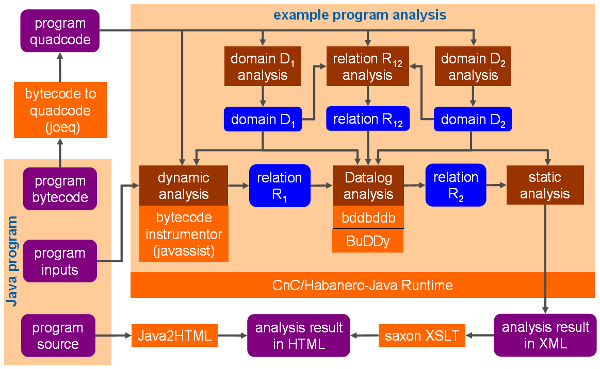
\includegraphics[scale=0.7]{chord_arch.png}}
\htmlonly{{\htmlimg{chord_arch.png}}}
\caption{Architecture of Chord}
\end{label}
\end{center}
\end{figure}

\subsubsection*{Chord Properties}

All inputs to Chord are specified by means of system properties. 
Chapter \ref{chap:properties} describes how to set properties and the meaning of 
each property that is recognized by Chord.

The Java program to be analyzed is also specified via properties.
These properties are described in Section \ref{sec:program-props}.
Chord analyzes Java bytecode, not Java source code, and therefore only requires
the program's class files.  Certain analyses, however, present
their results at the Java source level and therefore require the program's
Java source files as well.

\subsubsection*{Java Program Representation}

Chord uses the \xlink{Joeq}{http://joeq.sourceforce.net/} Java compiler framework
to convert Java bytecode, one class file at a time, into an intermediate representation called quadcode
that is more suitable for analysis. Chapter \ref{chap:program-representation}
describes the quadcode representation in detail.

\subsubsection*{Computing Analysis Scope}

A pre-requisite to analyzing a Java program using any program analysis framework, including Chord, is
to compute the {\it analysis scope}: the set of methods of the program to be analyzed.  Chord implements
several standard scope construction algorithms from the literature that differ in aspects such as
scalability, precision, and usability for the problem at hand.  Chapter \ref{chap:computing-scope}
describes these algorithms in detail.

\subsubsection*{Writing and Running Analyses}

Chord provides various {\it analysis templates}: classes containing boilerplate code that can be
extended by users to rapidly prototype different kinds of analyses.  An example is class RHSAnalysis,
named after [Reps, Horowitz, and Sagiv 1995], which can be extended by users to write a summary-based inter-procedural
context-sensitive static analysis by merely specifying the abstract domain and intra-procedural transfer functions.
Another exampls is DynamicAnalysis, which can be extended by
users to write a dynamic analysis by merely specifying which of various provided events to instrument, and
the transfer functions for those events.

A distinctive aspect of Chord is that each analysis is written modularly, independent of other analyses, along with lightweight
annotations specifying the inputs and outputs of the analysis.
Users must provide a unique name to each analysis, which allows the desired analyses to be called from the
command-line, via a property named \code{chord.run.analyses}.
Chord's runtime automatically computes
producer-consumer relationships between analyses (e.g., determines which analysis produces as output a
result that is needed as input by another analysis).  Before running a desired analysis,
Chord recursively runs other analyses until the inputs to the desired analysis have been computed; it
finally runs the desired analysis to produce the outputs of that analysis.

Chord can be invoked in one of two modes: classic or modern (depending upon whether the value of property
\code{chord.classic} is \code{true} (default) or \code{false}, respectively).
These two modes defer in the semantics of dependencies between analyses.  In particular, the classic mode
is simpler to understand for novice users (the dependencies are only data dependencies) but has a sequential
runtime, whereas the modern mode is harder to understand (there are both data and control dependencies)
but has a parallel runtime that is capable of running analyses without dependencies between
them in parallel.  The parallel runtime is based on \xlink{Habanero-Java}{http://habanero.rice.edu/hj.html},
and the semantics of the dependencies between analyses is based on the
\xlink{Habanero Concurrent Collections (CnC)}{http://habanero.rice.edu/cnc.html} declarative parallel
programming model.

Chapter \ref{chap:analyses} describes the various analysis templates and how to connect disparate analyses
together via dependencies in either of the above two modes.

\subsubsection*{Dynamic Analysis}

Chord uses the \xlink{Javassist}{http://www.javassist.org/} Java bytecode manipulation
framework for instrumenting bytecode and doing dynamic analysis.
Chord offers the most versatile capabilities of any existing dynamic analysis framework
for Java, particularly the ability to instrument the entire JDK (including classes in
package java.lang).
Specifically, it includes support for:
\begin{itemize}
\item
offline as well as load-time instrumentation of Java bytecode;
\item
processing of dynamic analysis events online in the same JVM or offline in a different JVM with an uninstrumented JDK (the latter circumvents performance and correctness problems that can arise if a single JVM with an instrumented JDK is used to generate and handle events); and
\item
allowing the event-generating and event-handling JVMs to run either serially (by storing the entire trace of events to a regular file) or in parallel (by streaming the trace of events in a piped file).
\end{itemize}
Chapter \ref{chap:dynamic-analysis} describes all aspects of dynamic analysis in Chord.

\subsubsection*{Datalog Analysis}

An analysis in Chord can be written either imperatively in Java or declaratively in Datalog.
Chord uses the BDD-based Datalog solver \xlink{bddbddb}{http://bddbddb.sourceforge.net/} to
run analyes written in Datalog.
Chapter \ref{chap:datalog-analysis} describes all aspects of Datalog analysis.

%If the analyses are purely static, it suffices to specify the main class of the program
%(via property \code{chord.main.class}) and the application classpath of the program (via property \code{chord.class.path}).
%If the analyses need to present their results at the Java source level, then
%the path of the program's Java source files is also required (via property \code{chord.src.path}).
%Finally, if any analysis is dynamic, then the command-line arguments to be used for running the
%program must also be specified (via property \code{chord.run.ids} and properties \code{chord.args.<N>} for
%each item \code{<N>} in the value of property \code{chord.run.ids}).
